%%%%%%%%%%%%%%%%%%%%%%%%%%
% SECTION :: IR examples %
%%%%%%%%%%%%%%%%%%%%%%%%%%
\section{IR Introductory Example}
%%%%%%%%%%%%%%%%%%%%%%%%%%%%%
% Frame Open :: IR examples %
%%%%%%%%%%%%%%%%%%%%%%%%%%%%%
\frame{\frametitle{IR Introductory Example}
\begin{itemize}
\item Consider the simple expression: \textit{32765+8}.
\item IR is produced by scanning the AST recursively as follows:
\begin{itemize}
\item First, the left subtree (a leaf actually) is scanned,
      producing the IR command: \textbf{li Temp\_29, 32765}.
\item Then, the right subtree (a leaf too) is scanned,
      producing the IR command: \textbf{li Temp\_30, 8}.
\item Finally, the binop father node uses the temporaries
      returned from its operand sons to produce the IR command:\\
      \textbf{add Temp\_31, Temp\_29, Temp\_30}.
\end{itemize}
\begin{figure}[htbp]
\begin{center}
% Requires \usepackage{graphicx}
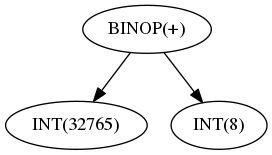
\includegraphics[width=4.0cm]{AST.png}\\
\label{Figure_Simple_Addition_Of_2_Integers_AST}
\end{center}
\end{figure}
\item Note that the IR recursive scan of the AST
      resembles the scan performed by the semantic analyzer.
      However here expression subtrees return their temporary,
      not their type.
\end{itemize}
%%%%%%%%%%%%%%%%%%%%%%%%%%%%%%%%%%%
% Frame Close :: Warm up examples %
%%%%%%%%%%%%%%%%%%%%%%%%%%%%%%%%%%%
%%%%%%%%%%%%%%%%%%%%%%%%%%%%%%%%%%%
% Frame Close :: Warm up examples %
%%%%%%%%%%%%%%%%%%%%%%%%%%%%%%%%%%%
}